\section{C2 EXTERNAL DATA REPRESENTATION, Presentation Layer} 
\rtext{Heterogeneity}
HW: Diff. HW architectures store bytes:Big, Small Endian
ProgrammingLanguage:Diff. PL store data types differently:AB, 0AB
\rtext{Transformation between representations}: Transformation between local and remote representations|Information may lost
\textbf{Two realizations}:
$1.$\textbf{Pairwise transformation between $n$ local representations}(vollständigGraph,$\#n^2 - n$, Either sender or receiver has to transform) 
$2.$\textbf{Transformation to and from canonical representation}(a single canonical $C$ as intermediate representation|No local information about communication
partner needed| $\#2*(n-2)$, $ -2$if canonical is one of $n$)
\rtext{XDR} partOf NFS, OSPresentationLayer, encodes only data items, no meta information about their types +:easy, -:Receiver lost data description
\textbar exactly 32 bit integer is stored according to \textbf{big endian} +:Fixed length reduces computation. -:wasting
\textbar Data is encoded into blocks of multiples of 4: n-bytes contain data; r-bytes are used for padding with n + r mod 4 = 0
\textbar int: int32; float=Sign+Exponent+Mantissa, String=length\_int32+bytes, array=length\_int32+ele
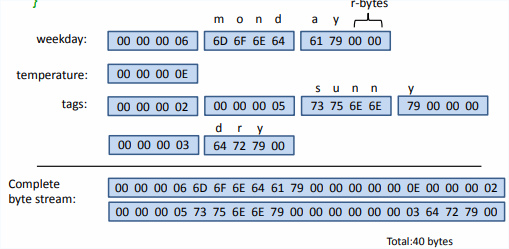
\includegraphics[width=.8\linewidth]{chap2_2.png} 
\lstinline{struct forecast:String weekday;int temperature;String tags<>;}
\rtext{ASN.1}:Abstract description of data types,telecommunication,internet protocol 
\textbar Enables exchange in heterogeneous systems
\textbar \btext{abstractSyntax $\overset{compiler}{\rightarrow}$ concreteSyntax Java, C++, they transfer syntax using encodingRules}
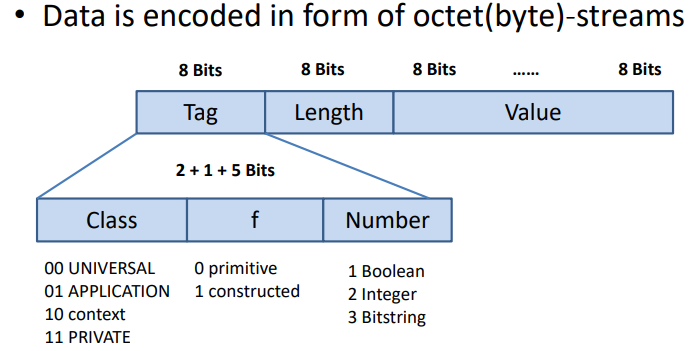
\includegraphics[width=.45\linewidth]{chap2_3.png}
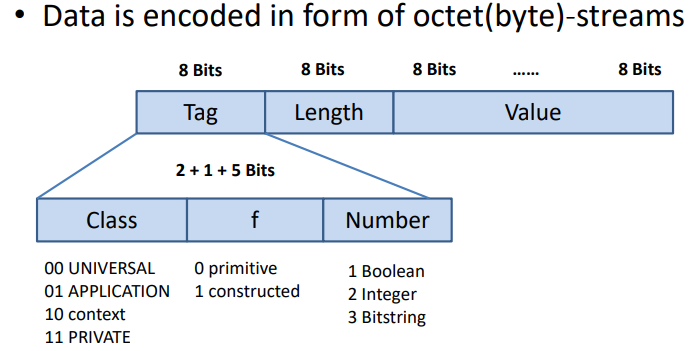
\includegraphics[width=.45\linewidth]{chap2_4.png}
\lstinline{Forecast::==SET{weekday IA5String,temperature Interger,tags SEQUENCE OF IS5String;}
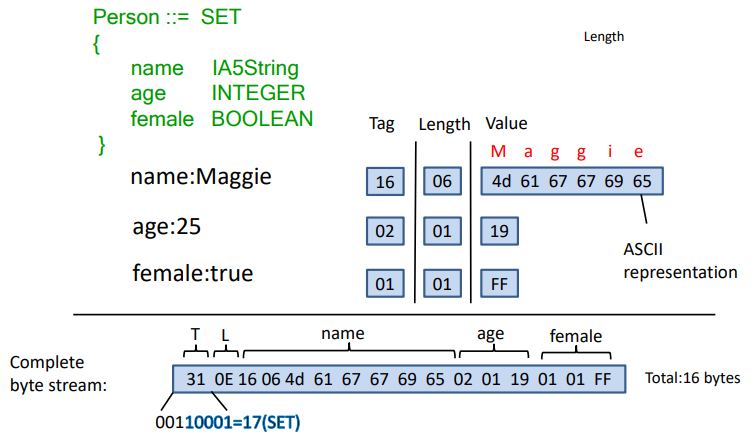
\includegraphics[width=.45\linewidth]{chap2_5.png}
\textbar encodes type information, +:receiver not need to know data description,-:additional overhead
\rtext{Java object serialization,JOS}
Stream-based transmission of serialized objects(Via TCP or UDP sockets)
, Receiver of object needs implementation of class
, Serialization does not require class specific code(Java reflection)
, Class implements java.io.Serializable interface
\textbf{-}: locked into Java(No support for heterogeneous systems), No support for versioning(If the serialized class changes, all network nodes
have to be updated)
\rtext{serialize:obj2bit}\lstinline{Socket s = new Socket("localhost", 8022);ObjectOutputStream oos = new ObjectOutputStream(s.getOutputStream()); oos.writeObject(obj);}
\rtext{deserialize:bit2obj}\lstinline{ServerSocket ss = new ServerSocket(8022);Socket s = serverSocket.accept();ObjectInputStream ois = new ObjectInputStream(s.getInputStream());obj=(Obj)ois.readObject();}
\rtext{XML}De facto standard for data exchange
\textbar Schema: \lstinline{<xsd:element name="forecast"> <xsd:complexType> <xsd:all> <xsd:element name="weekday" type="xsd:string"/> <xsd:element name="temperature" type="xsd:integer"/> <xsd:element name="tags">
<xsd:complexType> <xsd:sequence> <xsd:element name="tag" type="xsd:string" maxOccurs=\"unbounded\"/> </xsd:...>}
\textbar \lstinline{<forecast> <weekday>monday</weekday> <temperature>14</temperature> <tags> <tag>sunny</tag> <tag>dry</tag> </..>}
\rtext{JSON} human-readable text to transmit data objects
\textbar \lstinline{{"forecast":{"weekday":"monday","temperature" :14,"tags":["sunny","dry"] }\}\}}
\textbar \textbf{+ XML/JSON}:readable, defined as standard, JS support JSON(directly loaded  Browser and deserialized)
\textbar \textbf{- XML/JSON}: verbose, badPreformance, longOverhead, slowWriteParse
\rtext{ProtocolBuffersGoogle}: Similar concept like ASN.1, but not standard, efficient binary serialization, heterogeneous systems
\btext{data structures defined in .proto file(IDL) generate serialization code(Java, C$\#$), then java, .NET projects request, response each other}
\textbar DataModel.proto: \lstinline{message forecast{required string weekday =1;required int32 temperature =2;repeated string tags =3; optional float price=4;}\}}
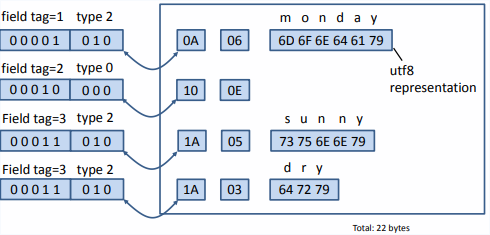
\includegraphics[width=.45\linewidth]{chap2_6.png}
\textbar RPC ServiceInterface.proto: \lstinline{enum Status{OK=0;EXISTING=1;NOT_EX=2;ERROR=3;}} \lstinline{message SearchRequest{required String attribute =1;required String value =2;}} \lstinline{message CustomerList{repeated Customer customers =1;}}
\lstinline{service AdministrationService{rpc CreateCustomer (Customer) return (Status); rpc DeleteCustomer(Customer) return (Status); rpc SearchCustomer(SearchRequest) return (CustomerList);}}

\textbar \textbf{+:}efficient writing/parsing,well documented,Versioning \textbf{-:}No RPC
\rtext{ApacheThrift:framwork, applied Hadoop and HBase}
.thrift: \lstinline{struct Forecast{1: string weekday 2: i32 temperature 3: list<string> tags}\}}
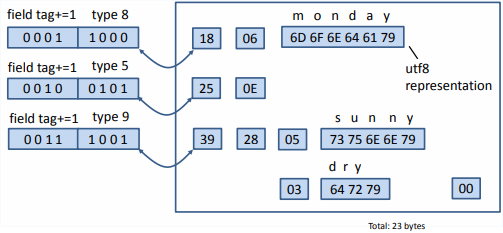
\includegraphics[width=.45\linewidth]{chap2_7.png}
\textbar \textbf{+:}Multiple protocols to serve different purposes(binary, JSON),RPC,Open source,widely,Versioning
\rtext{VariableLength:}